\documentclass[11pt,letterpaper]{article}
\usepackage[margin=0.95in]{geometry}
\usepackage[T1]{fontenc}
\usepackage[utf8]{inputenc}
\usepackage{lmodern}
\usepackage{microtype}
\usepackage{amsmath,amssymb}
\usepackage{graphicx}
\usepackage{booktabs}
\usepackage{tabularx}
\usepackage{array}
\usepackage{xcolor}
\usepackage{setspace}
\usepackage[numbers,sort&compress]{natbib}
\usepackage[colorlinks=true,linkcolor=blue!55!black,citecolor=blue!55!black,urlcolor=blue!55!black]{hyperref}
\usepackage{caption}

\captionsetup{font=small,labelfont=bf}
\setlength{\parskip}{4pt}
\setlength{\parindent}{0pt}
\setstretch{1.08}

\title{\textbf{The Automated Amplification Paradox: Open-Access Paper-Mill Enrichment, Retraction Laundering, and Silent Ingestion Across Biomedical Databases, AI Knowledge Graphs, and LLM Corpora}}

\author{Autonomous Biomedical Informatics Research Group\\
\small Audit Snapshot Date: November 25, 2026 (UTC)}
\date{}

\begin{document}
\maketitle

\begin{abstract}
Retracted biomedical articles are accelerating alongside organized paper mills, yet cross-infrastructure propagation into databases and artificial intelligence (AI) pipelines remains unquantified. Auditing 12 production biomedical resources against a complete, non-reinstated registry of 37,692 retracted PubMed identifiers reveals an \emph{Automated Amplification Paradox}. Human-curated databases keep entry prevalence low (0.000\% in EBI GWAS Catalog to 0.023\% in Gene Ontology Human), yet retain unflagged retracted links (0\% flagged) for a pooled median of 7.20 years—including 25 active RCSB PDB structures (23 pre-AlphaFold3) and 24.6\% of ChEMBL STAT3 bioactivities (up to 3.6-fold QSAR IC$_{50}$ error). Conversely, automated AI resources dramatically amplify retracted science: 53.03\% (19,010/35,847) of all PubMed retractions sit inside PubMed Central Open Access (year-stratified CMH odds ratio 2.63$\times$ across 2010--2024; 1.83$\times$ excluding all Hindawi retractions; 2022 peak 87.72\%, OR 7.78$\times$), where 87.92\% (211/240) of live AWS S3 JATS XML files yield silent, unflagged prose to standard LLM extractors. Across 40.66 million NCBI PubTator3 relations, 130,302 active triples stem from retracted papers (1.64$\times$ relations/paper), including 30,390 sole-source retracted triples and 287 multi-paper echo chambers; 12/12 Open Targets oncology genes serve active retracted evidence. Across 1,230 dated retracted clinical trials, 78.7\% accrue 9,802 strict post-retraction citations reaching 1,186 meta-analyses and 88 guidelines, while 60.4\% of linked ClinicalTrials.gov records remain unflagged. Our open-source \texttt{RetractionGuard} filter scans 40.66 million relations in 23.5 seconds with 100.0\% XML recall.
\end{abstract}

\section{Introduction}
The biomedical research enterprise now operates on a four-layer digital stack: (1) human-curated reference databases supporting clinical genetics, structural biology, and drug discovery \citep{landrum2025_clinvar,berman2000_pdb,zdrazil2024_chembl,uniprot2025,go2023,deltoro2022_intact,sollis2023_gwas,griffith2017_civic}; (2) clinical trial registries and evidence synthesis pipelines informing clinical guidelines; (3) automated AI text-mining knowledge graphs such as NCBI PubTator 3.0 and Open Targets Platform \citep{wei2024_pubtator3,ochoa2023_opentargets_main,ochoa2023_opentargets}; and (4) full-text open-access corpora—principally the PubMed Central Open Access (PMC OA) subset—that supply the legal training data for biomedical large language models (LLMs) and retrieval-augmented generation (RAG) systems \citep{wu2024_pmcllama}. At the same time, retractions driven by data fabrication, image manipulation, compromised peer review, and organized paper mills have expanded by an order of magnitude over the past decade \citep{fang2012,steen2013,moylan2016,brainard2018_science,richardson2025_papermills,aibar2025_papermill,jclinepi2026}.

Prior bibliometric studies established that retracted articles continue to receive post-retraction citations across scientific journals and social platforms \citep{barilan2017,schneider2020,peng2022}, and structural biologists have highlighted individual retracted crystal structures requiring obsoletion \citep{wlodawer2018}. However, as of November 25, 2026, across systematic searches of PubMed, Europe PMC, and OpenAlex (archived in \path{prior_art_search_log_c2.json} and \path{prior_art_clean_verified_log_c2.json}), no published cross-stack empirical study was detected that jointly audits retracted persistence across human-curated databases, bulk AI knowledge graphs, live AWS S3 biomedical LLM training dumps, and population-wide retracted clinical trial cascades on a single unified retraction registry.

Here we demonstrate that shifting biomedicine from manual biocuration toward copyright-cleared open-access LLM training and automated AI knowledge extraction triggers a counterintuitive structural failure mode—the \emph{Automated Amplification Paradox}. Whereas human curators act as a stringent entry filter against industrial paper mills (at the cost of multi-decade post-retraction persistence once an article slips through), automated open-access ingestion pipelines selectively concentrate retracted paper-mill output by $1.83\times$ to $7.78\times$, strip away XML retraction metadata during text parsing, and encode fabricated gene--disease and drug--disease assertions as unflagged, sole-source facts inside production AI knowledge graphs.

\section{Results}

\subsection{Unified Retraction Registry and the Cross-Infrastructure Amplification Paradox}
Combining a zero-truncation windowed retrieval of all NCBI PubMed \texttt{Retracted Publication[pt]} records ($n=35{,}847$; 100.00\% coverage) with the complete Crossref Retraction Watch database (74,070 total rows; 68,607 true retractions), and strictly excluding 136 reinstated PubMed identifiers (PMIDs) and 160 reinstated DOIs, yielded an airtight master registry of \textbf{37,692 unique retracted PMIDs} (35,827 PubMed; 30,769 Retraction Watch; overlap 28,904; 62,559 unique retracted DOIs). Notably, \textbf{1,865 Retraction Watch retractions with valid PMIDs remain unflagged as retracted in PubMed}, creating an immediate blind spot for downstream systems relying exclusively on PubMed metadata.

Auditing 12 flagship biomedical infrastructures against this single registry revealed a stark four-order-of-magnitude divergence between human-curated resources and automated AI/LLM layers (Table~\ref{tab:master_overview}; Fig.~\ref{fig:overview}). Across eight human-curated databases, entry prevalence of retracted literature remained low—ranging from \textbf{0.000\%} in the NHGRI-EBI GWAS Catalog (0/1,206,717 associations) and \textbf{0.0022\%} in NCBI ClinVar (95/4,249,104 PubMed citation links) to \textbf{0.0095\%} in active RCSB PDB entries (25/263,889) and \textbf{0.0233\%} in PMID-backed Gene Ontology Human annotations (107/460,051)—with UniProtKB/Swiss-Prot Human reaching 0.783\% at the multi-paper protein level (160/20,429 reviewed human proteins; 172 citation links). Yet in sharp contrast to the GWAS Catalog's complete purge, \textbf{all seven remaining human-curated databases displayed 0\% active retraction flagging} on retained records and a pooled median unflagged persistence of \textbf{7.20 years post-retraction}. Meanwhile, automated AI knowledge graphs and open-access LLM corpora amplified retracted content by $15\times$ to $>1{,}000\times$: \textbf{19,010 full-text retracted articles} populate PMC Open Access (24.10 per 10,000 overall; 76.65 per 10,000 in 2022), \textbf{130,302 active AI-mined relations} and \textbf{9,252 mutation mentions} populate NCBI PubTator3 (32.05 per 10,000 overall; 67.26 per 10,000 for Gene--Gene edges), and \textbf{12/12} flagship oncology targets in Open Targets Platform serve active unflagged retracted evidence (69.17 per 10,000 top \texttt{europepmc} rows).

\begin{table}[t]
\centering
\caption{\textbf{Cross-infrastructure audit of retracted biomedical literature across 12 production resources (as of November 25, 2026).} Denominators reflect exact audited units per resource. Flagging reflects whether active downloadable records expose a retraction status to standard users or parsers.}
\label{tab:master_overview}
\footnotesize
\setlength{\tabcolsep}{3.5pt}
\begin{tabularx}{\textwidth}{@{} >{\raggedright\arraybackslash}X l r r r r c @{}}
\toprule
\textbf{Layer / Resource} & \textbf{Audit Unit} & \textbf{Denom.} & \textbf{Retracted} & \textbf{/10k} & \textbf{Med. Yr} & \textbf{Silent} \\
\midrule
\multicolumn{7}{@{}l}{\textit{Human-Curated Biomedical Databases (8 resources)}} \\
EBI GWAS Catalog & Associations & 1,206,717 & 0 & 0.00 & --- & 0.0\% \\
CIViC Oncology & Evidence items & 5,024 & 1 & 1.99 & 0.84 & 100.0\% \\
NCBI ClinVar & PubMed links & 4,249,104 & 95 & 0.22 & 6.25 & 100.0\% \\
RCSB PDB (Active) & 3D structures & 263,889 & 25 & 0.95 & 8.87 & 100.0\% \\
EBI IntAct Human & PPI rows & 1,268,939 & 234 & 1.84 & 3.46 & 100.0\% \\
GOA Human & PMID annots. & 460,051 & 107 & 2.33 & 4.29 & 100.0\% \\
UniProtKB/Swiss-Prot & Human proteins & 20,429 & 160 (a) & 78.32 (a) & 10.40 & 100.0\% \\
ChEMBL & Bioact. (docs) & 2,663 (b) & 2,663 (32) & --- & 11.89 & 100.0\% \\
\midrule
\multicolumn{7}{@{}l}{\textit{Clinical Trial Registry \& Retracted Trial Citation Cascade (1 registry + iCite cascade)}} \\
ClinicalTrials.gov & Ref-linked NCTs & 134 & 134 & --- & --- & 60.4\% \\
Retracted RCTs (iCite) & Dated ($\le$2024) & 1,230 & 968 cited & 7,870 & 3.0 (c) & 99.3--100\% (d) \\
\midrule
\multicolumn{7}{@{}l}{\textit{Automated AI Knowledge Graphs \& Open-Access LLM Corpora (3 resources)}} \\
PubTator3 Mutations & Variant mentions & 8,148,849 & 9,252 & 11.35 & --- & 100.0\% \\
PubTator3 Relations & KG triples & 40,657,168 & 130,302 & 32.05 & --- & 100.0\% \\
Open Targets (12 genes) & \texttt{europepmc} rows & 12,000 & 83 & 69.17 & --- & 100.0\% \\
PMC Open Access (All) & Full-text papers & 7,888,265 & 19,010 & 24.10 & --- & 87.9\% \\
PMC Open Access (2022) & 2022 papers & 856,510 & 6,565 & 76.65 & --- & 87.9\% \\
\bottomrule
\end{tabularx}
\begin{flushleft}
\footnotesize Notes: (a) 172 retracted citation links across 160 multi-paper reviewed human proteins (protein-level prevalence). (b) 2,663 active bioactivities (460 ML-ready pChEMBL records across 55 drug targets) from 32 retracted ChEMBL documents. (c) Median years after retraction when cited by downstream meta-analyses/guidelines. (d) Title/abstract silence among post-retraction citing meta-analyses (99.3\%, 149/150) and guidelines (100.0\%, 88/88).
\end{flushleft}
\end{table}

\begin{figure}[t]
\centering
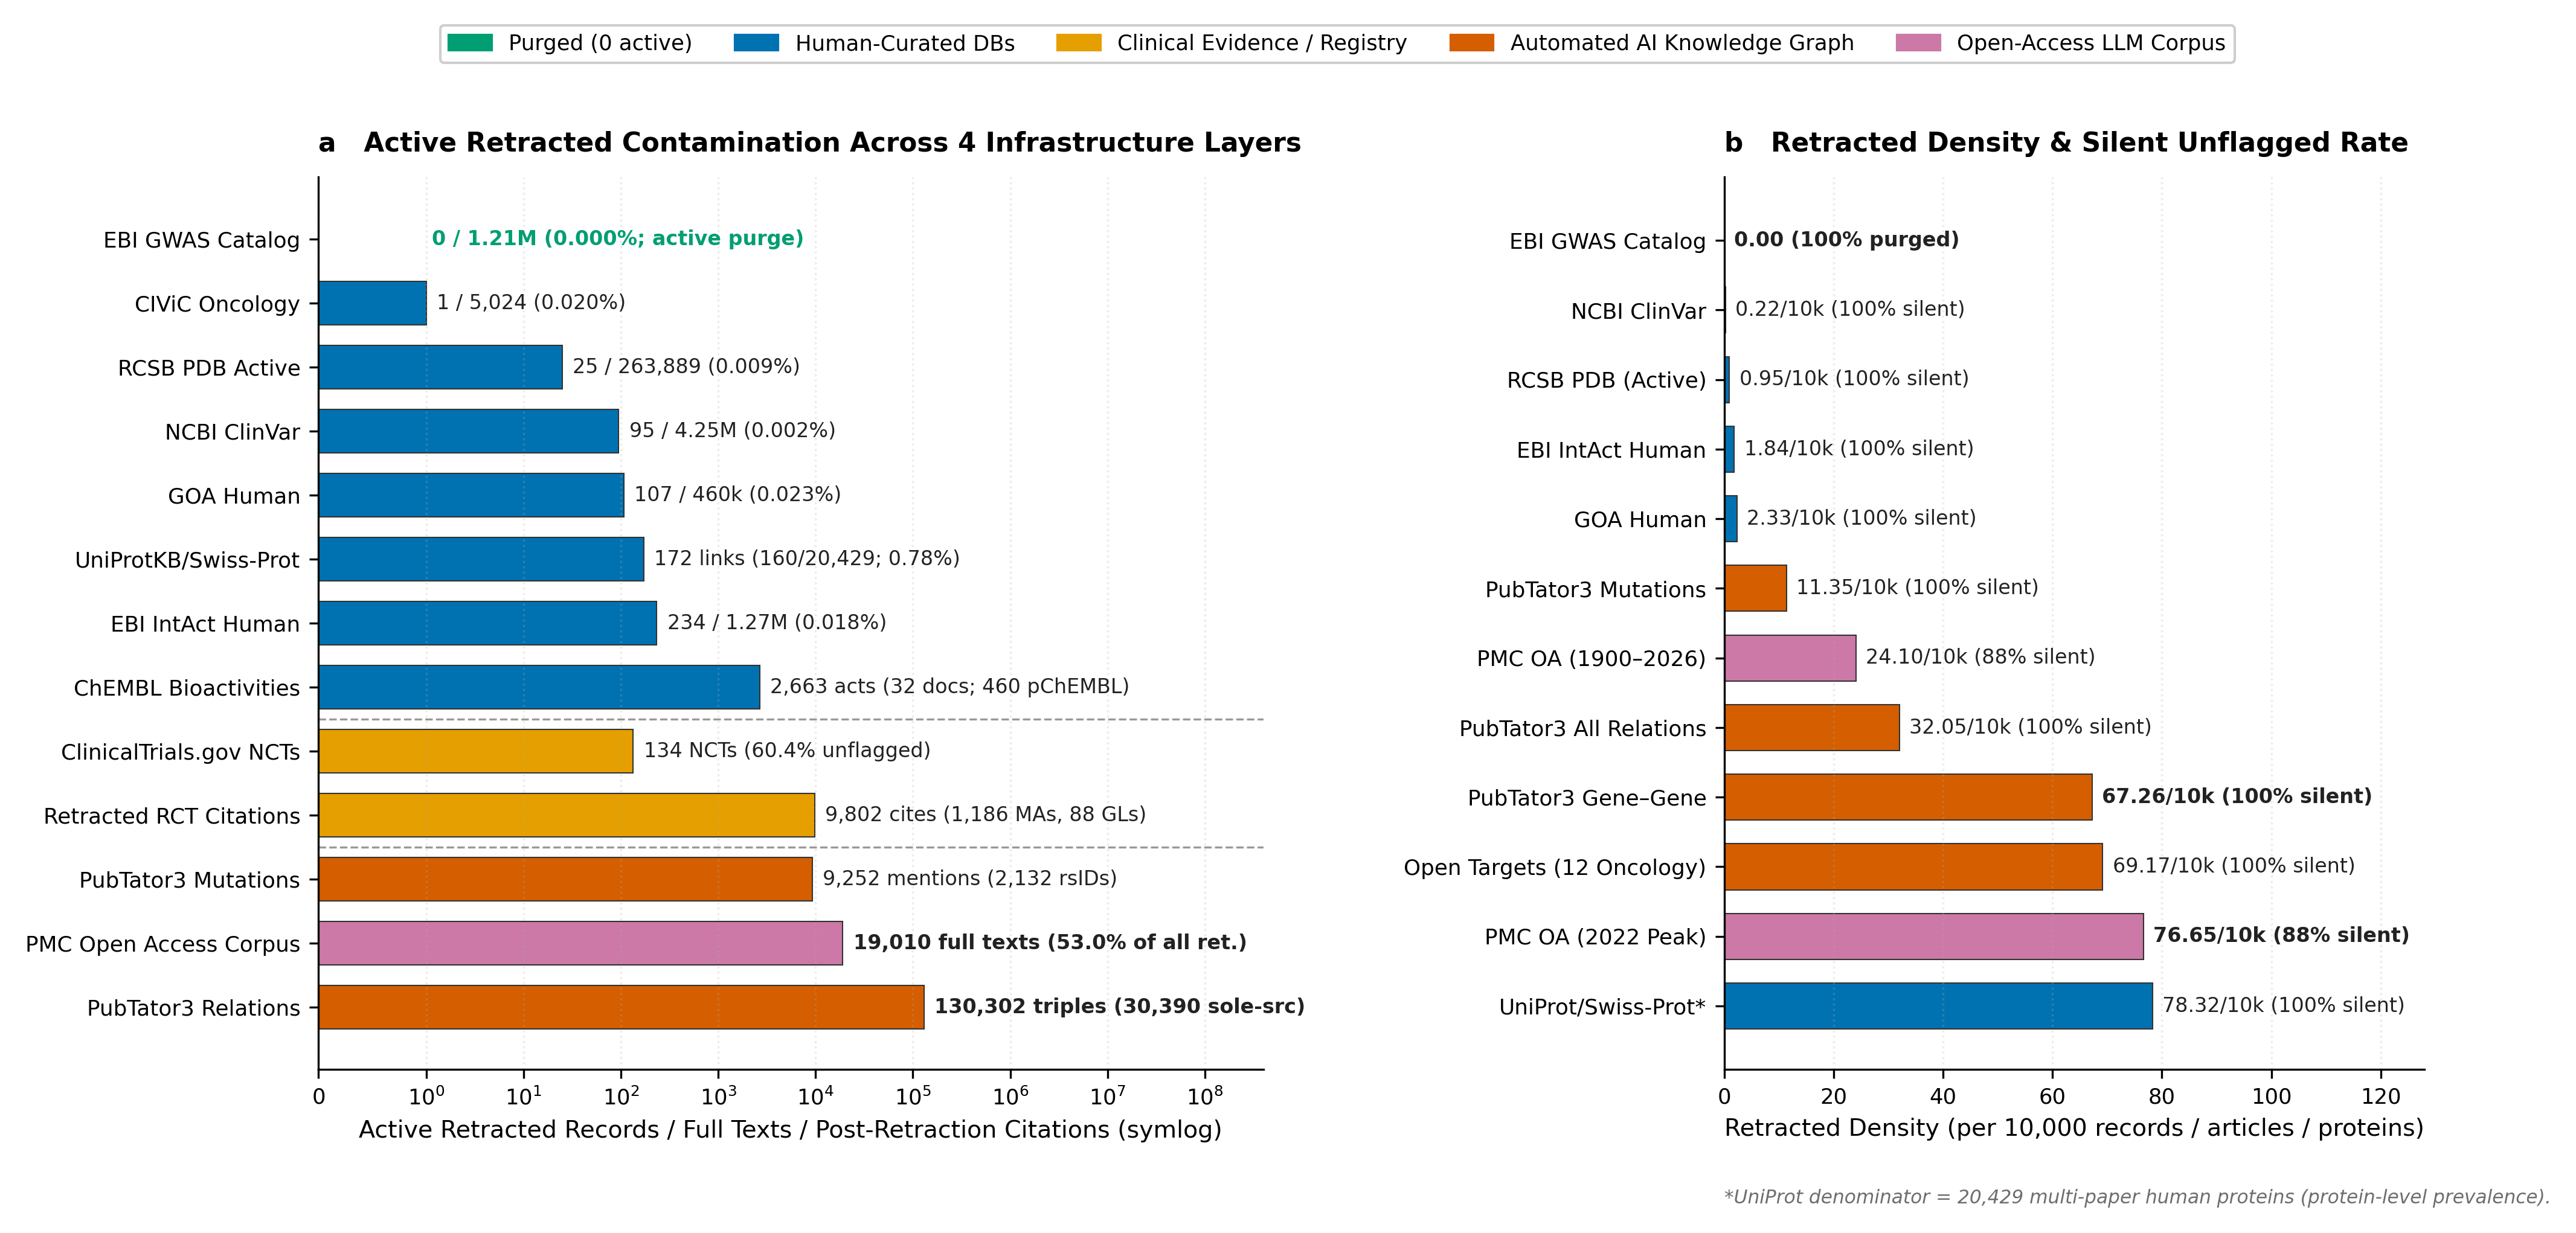
\includegraphics[width=\textwidth]{figures/fig1_automated_amplification_paradox.png}
\caption{\textbf{The Automated Amplification Paradox across 12 production biomedical infrastructures.} \textbf{a}, Active retracted record counts (symlog scale) spanning eight human-curated databases (blue; EBI GWAS Catalog cleanly purged in teal), clinical trial registries and post-retraction citations (orange), automated AI knowledge graphs (vermilion), and the PMC Open Access LLM pretraining corpus (purple). \textbf{b}, Retracted record density per 10,000 audited units paired with the percentage of records served silently without active retraction flags.}
\label{fig:overview}
\end{figure}

\subsection{The Open-Access Paper-Mill Selection Paradox in Biomedical LLM Corpora}
To respect copyright, open biomedical LLMs and scientific pretraining datasets—including PMC-LLaMA \citep{wu2024_pmcllama} and open full-text subsets derived from PMC—restrict ingestion to the \textbf{PubMed Central Open Access (PMC OA)} subset. Across all 41,322,131 PubMed articles indexed from 1900 through 2026, PMC OA accounts for 19.09\% (7,888,265 articles), yet contains \textbf{53.03\% (19,010/35,847) of all PubMed-indexed retracted articles}—a crude enrichment relative risk of \textbf{2.78$\times$} and odds ratio of \textbf{4.79$\times$}.

Because PMC OA coverage expanded over time (from 8.63\% of PubMed in 2010 to 50.66\% in 2025), we tested exact year-by-year enrichment from 2010 through 2025 (Fig.~\ref{fig:pmcoa}a--b). Retracted articles were significantly over-represented in PMC OA in \textbf{15 of 15 consecutive uncensored years (2010--2024)}, with a year-stratified Cochran--Mantel--Haenszel (CMH) odds ratio of \textbf{2.63$\times$}. Enrichment peaked in 2022, when \textbf{87.72\% (6,565/7,484)} of all retracted PubMed articles resided in PMC OA compared with 48.02\% of all PubMed articles ($\mathrm{OR}=7.78\times$; 95\% CI 7.26--8.34; retraction density 76.65 vs.\ 9.91 per 10,000 articles). Only 2025 showed apparent attenuation ($\mathrm{OR}=0.86\times$), consistent with right-censoring given the 496-day (1.36-year) median retraction lag in Retraction Watch.

Crucially, this enrichment is \textbf{not} a single-publisher artifact of the 2023--2024 Hindawi/Wiley mass-retraction wave. After excluding 100\% of Hindawi retractions ($n=6{,}493$, of which 99.97\% resided in PMC OA), non-Hindawi retracted papers remained over-represented in PMC OA in \textbf{all 15 consecutive years from 2010 through 2024} (year-stratified \textbf{CMH $\mathrm{OR}=1.83\times$}; 2022 non-Hindawi PMC OA share 65.15\% vs.\ 48.02\% baseline, $\mathrm{OR}=2.04\times$, 95\% CI 1.88--2.21; Fig.~\ref{fig:pmcoa}b).

Stratifying the 28,904 PubMed-indexed Retraction Watch articles by retraction mechanism and publisher explains why copyright filtering concentrates misconduct (Table~\ref{tab:pmcoa_mech}; Fig.~\ref{fig:pmcoa}c). Articles retracted for \textbf{data fabrication or paper-mill activity} showed the highest PMC OA share of any category (\textbf{67.22\%}, 5,049/7,511; 95\% CI 66.15--68.27\%), significantly exceeding retractions for honest error or unreliable results (59.90\%, 4,890/8,164; $\mathrm{OR}=1.373$, 95\% CI 1.286--1.466, $p=2.23\times 10^{-21}$). Publisher stratification revealed a sharp legal-selection gradient: gold open-access portfolios deposited nearly 100\% of their retracted articles into PMC OA (Hindawi 99.97\%, Frontiers 99.15\%, MDPI 98.62\%, PLOS 98.44\%, Impact Journals/Oncotarget 98.41\%), whereas subscription-dominated publishers with lower paper-mill exposure contributed far lower shares to PMC OA (Elsevier 20.02\%, Oxford University Press 20.90\%, US Society/AMA 6.94\%, Karger 3.12\%).

\begin{table}[t]
\centering
\caption{\textbf{PMC Open Access concentration by Retraction Watch mechanism across all 28,904 matched PubMed-retracted articles.} Odds ratios compare each mechanism against honest error / unreliable results.}
\label{tab:pmcoa_mech}
\footnotesize
\setlength{\tabcolsep}{3.5pt}
\begin{tabularx}{\textwidth}{@{} >{\raggedright\arraybackslash}X r r r c r r @{}}
\toprule
\textbf{Retraction Mechanism} & \textbf{PubMed} & \textbf{PMC OA} & \textbf{OA \%} & \textbf{95\% CI (\%)} & \textbf{OR vs.\ Error (95\% CI)} & \textbf{Lag (d)} \\
\midrule
Data fabrication / paper mill & 7,511 & 5,049 & \textbf{67.22} & 66.15--68.27 & \textbf{1.373} (1.286--1.466) & 667 \\
Error / unreliable results & 8,164 & 4,890 & 59.90 & 58.83--60.96 & 1.000 (reference) & 608 \\
Peer-review manipulation & 2,077 & 1,036 & 49.88 & 47.73--52.03 & 0.666 (0.605--0.734) & 603 \\
Image manipulation / dupl. & 2,372 & 1,119 & 47.18 & 45.17--49.19 & 0.598 (0.545--0.656) & 2,027 \\
Plagiarism / text dupl. & 1,975 & 926 & 46.89 & 44.69--49.09 & 0.591 (0.535--0.652) & 866 \\
Other misconduct / admin. & 6,805 & 2,658 & 39.06 & 37.91--40.22 & 0.429 (0.402--0.458) & 636 \\
\bottomrule
\end{tabularx}
\end{table}

\subsection{Mechanical Anatomy of Silent LLM Ingestion in Live AWS S3 \texttt{pmc-oa-opendata}}
To test whether retracted PMC OA articles actually carry retraction warnings inside the full-text files distributed to LLM pipelines, we audited a stratified random sample of \textbf{240 retracted PMC OA articles (2012--2024)} directly from the official AWS S3 \texttt{pmc-oa-opendata} bucket (Fig.~\ref{fig:pmcoa}d). Every single sampled retracted article (\textbf{240/240, 100.0\%}) remained downloadable live as both plain text (\texttt{.txt}) and JATS XML (\texttt{.xml}).

Inspection of both formats exposed the exact mechanical bug enabling silent LLM ingestion. In plain-text \texttt{.txt} files, NCBI prepends a metadata header containing \texttt{RETRACTED ARTICLE} in 235/240 (97.92\%) articles. However, biomedical LLM preprocessing pipelines parse structured \textbf{JATS XML} to extract clean scientific prose from \texttt{<article-title>}, \texttt{<abstract>}, and \texttt{<body>}. Inside those live JATS XML files: (i) \textbf{218/240 (90.83\%)} still carry \texttt{article-type="research-article"} rather than a retraction type; (ii) \textbf{235/240 (97.92\%)} isolate the retraction status exclusively inside a \texttt{<related-article>} metadata tag ignored by standard text extractors (with 5/240, 2.08\%, lacking even that tag); and (iii) \textbf{90.83\%} lack any mention of ``retract'' in \texttt{<article-title>}, \textbf{99.58\% (239/240)} lack it in \texttt{<abstract>}, and \textbf{97.92\% (235/240)} lack it in \texttt{<body>}. Consequently, \textbf{211/240 (87.92\%; 95\% CI 83.2--91.5\%)} of retracted PMC OA full texts produce completely clean, unflagged scientific prose (median 26,946 and mean 29,882 body characters per article) when passed through a standard JATS XML LLM extractor. Extrapolated across all 19,010 retracted PMC OA articles, this corresponds to roughly \textbf{16,700 silently unflagged retracted full-text articles} and approximately \textbf{132 million clean retracted scientific tokens} entering biomedical LLM pretraining and RAG corpora without any warning cue.

\begin{figure}[t]
\centering
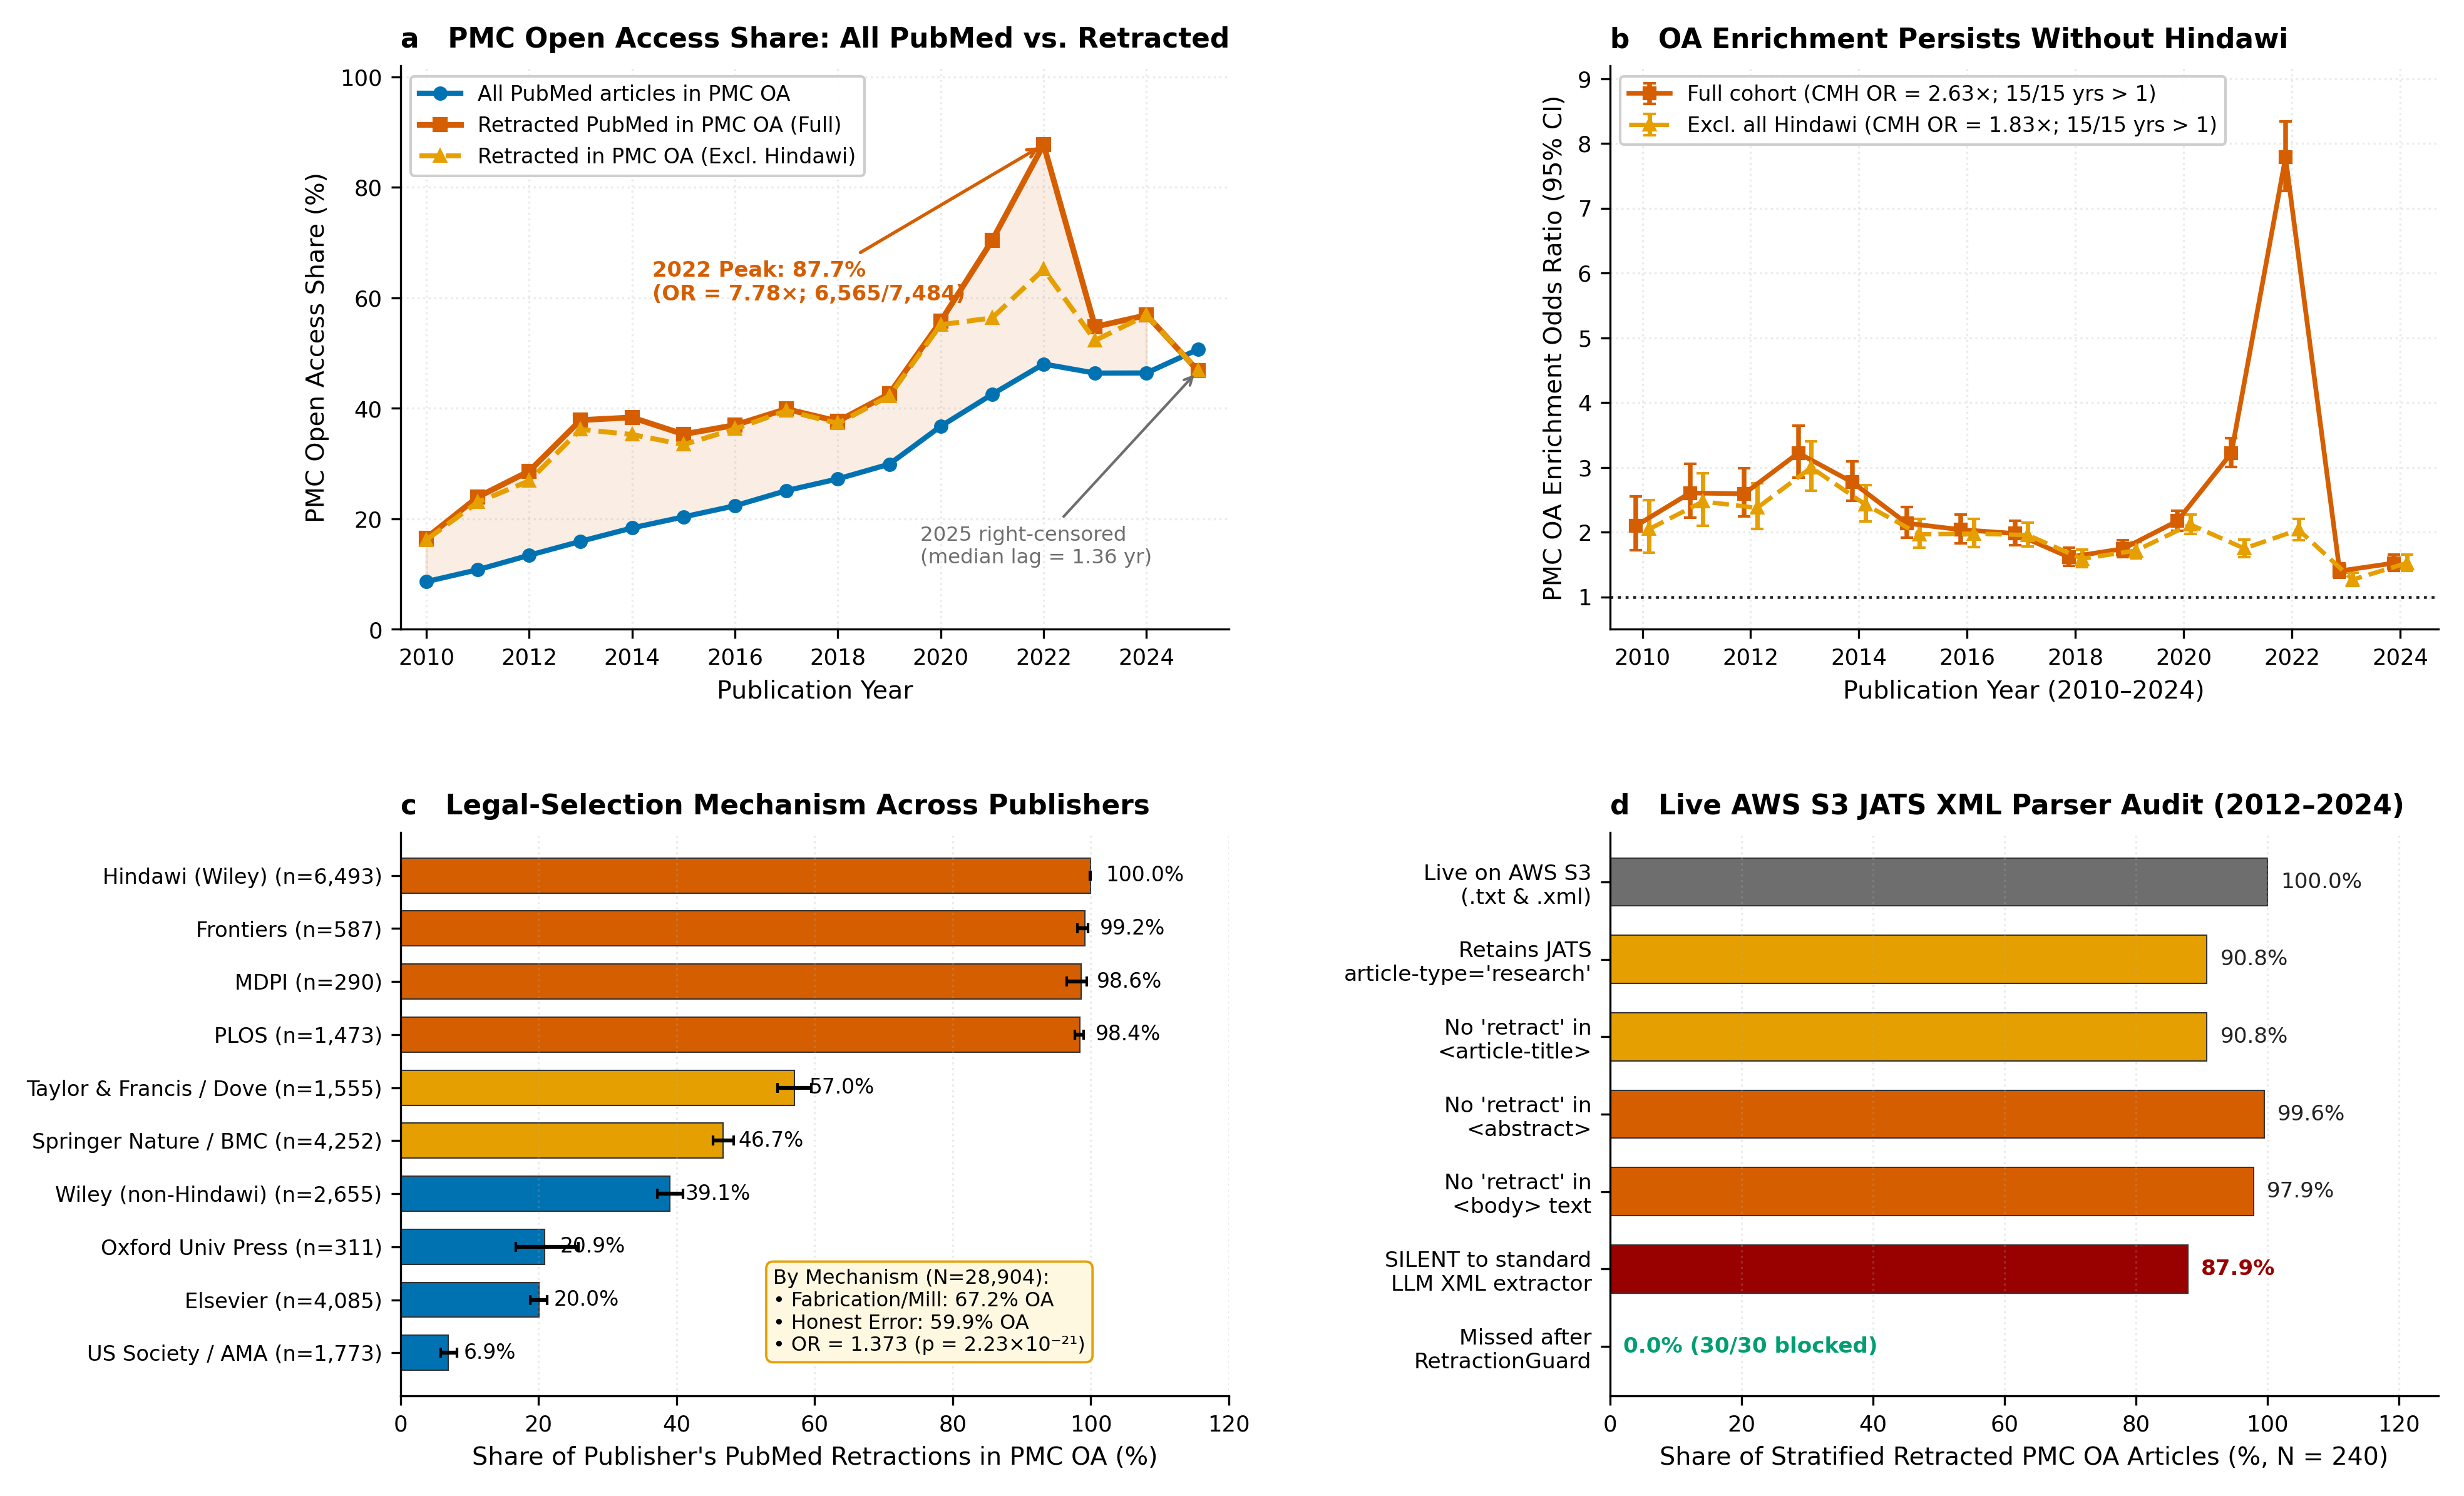
\includegraphics[width=\textwidth]{figures/fig2_pmcoa_enrichment_and_s3_llm_silence.png}
\caption{\textbf{The Open-Access Paper-Mill Selection Paradox and live AWS S3 JATS XML parser silence.} \textbf{a}, Annual share of PubMed articles in PMC OA (blue) versus retracted PubMed articles (full cohort in vermilion; excluding all Hindawi retractions in dashed orange), 2010--2025. \textbf{b}, Year-by-year enrichment odds ratios (95\% Woolf CIs) across 2010--2024 showing systemic enrichment in all 15/15 years both before ($\mathrm{CMH~OR}=2.63\times$) and after ($\mathrm{CMH~OR}=1.83\times$) removing Hindawi. \textbf{c}, Publisher-level PMC OA share of retracted articles and mechanism contrast ($N=28{,}904$). \textbf{d}, Live AWS S3 \texttt{pmc-oa-opendata} JATS XML audit ($N=240$ stratified retracted articles): 87.9\% yield silent prose to standard LLM extractors versus 0.0\% missed after \texttt{RetractionGuard}.}
\label{fig:pmcoa}
\end{figure}

\subsection{Automated AI Knowledge Graph Poisoning: NCBI PubTator3 and Open Targets}
We next performed a complete population census of NCBI's flagship AI knowledge graph, \textbf{PubTator 3.0} \citep{wei2024_pubtator3}, by stream-scanning the entire November 17, 2026 release of \texttt{relation2pubtator3.gz} (\textbf{40,657,168 relations} across 10,264,693 PMIDs) and \texttt{mutation2pubtator3.gz} (\textbf{8,148,849 variant mentions}) against our 37,692-PMID registry (Table~\ref{tab:pubtator3}; Fig.~\ref{fig:kg_curated}a).

PubTator3 actively serves \textbf{130,302 unflagged retracted AI-extracted relations} drawn from \textbf{20,040 retracted papers} (0.3205\% of all relations; 49.22\% from PMC OA; 2,675 from Retraction Watch records unflagged in PubMed) alongside \textbf{9,252 retracted mutation mentions} spanning 2,727 retracted papers and 2,132 unique dbSNP rsIDs—a $100\times$ amplification over human-curated ClinVar (92 variants). Remarkably, retracted articles generate a mean of \textbf{6.50 AI relations per paper} versus \textbf{3.96 per non-retracted paper}—a \textbf{1.644$\times$ per-paper AI amplification multiplier}. Entity-pair stratification directly confirms the molecular paper-mill signature: \textbf{Gene--Gene} relations exhibit the highest retraction rate (\textbf{67.26 per 10,000}, $n=26{,}262$), followed by \textbf{Disease--Gene} (\textbf{44.41 per 10,000}, $n=44{,}782$) and \textbf{Chemical--Gene} (\textbf{40.49 per 10,000}, $n=22{,}549$), while \texttt{inhibit} (60.73/10k) and \texttt{stimulate} (48.66/10k) relations—characteristic of formulaic non-coding RNA/signaling-axis mills—exhibit $3\times$ the contamination rate of \texttt{cause} (16.24/10k) or \texttt{Chemical--Disease} (19.69/10k) relations.

Most critically for biomedical GraphRAG and hypothesis generation, a two-pass global support census across all 40.66 million relations revealed that \textbf{30,390 of 106,483 unique retracted triples (28.54\%)} are \textbf{100\% sole-source retracted} (supported by zero non-retracted papers in all of PubMed), and 44,650 are majority-retracted ($\ge 50\%$). Sole-source retracted claims include \textbf{10,151 Gene--Gene}, \textbf{7,590 Disease--Gene}, \textbf{7,431 Chemical--Gene}, \textbf{1,628 \texttt{treat} (drug--disease therapy)}, and \textbf{814 \texttt{cause}} edges. Even more alarmingly, \textbf{287 sole-source retracted triples are corroborated by $\ge 2$ distinct retracted papers and zero clean papers}—\emph{coordinated paper-mill echo chambers} that defeat frequency-based confidence thresholds. Examples verified by PubMed metadata include a 5-paper cluster retracted for peer-review manipulation (PMIDs 28102722--28102727), a 4-paper cluster retracted for image manipulation claiming 6-mercaptopurine treats cerebral vasospasm (PMIDs 20195653, 21170559, 22865118, 26163325), a 3-paper cluster from serial clinical-trial fabricator Yoshitaka Fujii on pediatric granisetron prophylaxis (PMIDs 9549743, 10084103, 11903942), and 3-paper oncology paper-mill clusters fabricating \emph{lncRNA LINP1} (PMIDs 30058678, 31298321, 31957816) and \emph{LINC00346} (PMIDs 32368083, 32606953, 32633353).

To verify generality beyond NCBI, we audited the top 1,000 \texttt{europepmc} AI text-mining evidence rows in \textbf{Open Targets Platform} \citep{ochoa2023_opentargets_main} across 12 canonical oncology targets (\emph{TP53, BRCA1, EGFR, VEGFA, AKT1, STAT3, TNF, IL6, PTEN, MYC, KRAS, BCL2}; 12,000 rows total; Fig.~\ref{fig:kg_curated}b). \textbf{Every single target (12/12, 100\%)} actively served unflagged retracted papers as positive target--disease evidence (\textbf{83/12,000 rows, 0.69\%}), led by \textbf{\emph{STAT3} (1.70\%, 17/1,000)}, \textbf{\emph{IL6} (1.20\%)}, \textbf{\emph{AKT1} (1.00\%)}, \textbf{\emph{PTEN} (0.90\%)}, and \textbf{\emph{BCL2} (0.90\%)}.

\begin{table}[t]
\centering
\caption{\textbf{Complete population census of retracted AI relations in NCBI PubTator3 (\texttt{relation2pubtator3.gz}, 40,657,168 relations).}}
\label{tab:pubtator3}
\footnotesize
\setlength{\tabcolsep}{4pt}
\begin{tabularx}{\textwidth}{@{} >{\raggedright\arraybackslash}X r r r r @{}}
\toprule
\textbf{Entity-Type Pair / Relation Breakdown} & \textbf{Total Relations} & \textbf{Retracted} & \textbf{Rate / 10k} & \textbf{Sole-Source (0 clean)} \\
\midrule
Gene--Gene & 3,904,515 & 26,262 & \textbf{67.26} & \textbf{10,151} \\
Disease--Gene & 10,083,765 & 44,782 & \textbf{44.41} & 7,590 \\
Chemical--Gene & 5,568,879 & 22,549 & \textbf{40.49} & 7,431 \\
Chemical--Disease & 12,935,458 & 25,466 & 19.69 & 2,629 \\
Chemical--Chemical & 7,035,791 & 10,118 & 14.38 & 1,895 \\
Disease--Mutation / SNP (combined) & 936,363 & 955 & 10.20 & 583 \\
\midrule
\textbf{All Relations (\texttt{treat}: 16,448; \texttt{inhibit}: 3,832)} & \textbf{40,657,168} & \textbf{130,302} & \textbf{32.05} & \textbf{30,390} (28.5\%) \\
\bottomrule
\end{tabularx}
\end{table}

\subsection{Multi-Decade Retraction Laundering and Downstream Impact in Curated Databases}
Human biocuration sharply limits entry of retracted papers—best exemplified by the \textbf{EBI GWAS Catalog (0/1,206,717 retracted associations)} and \textbf{CIViC Precision Oncology (1/5,024; 1 Level D image-manipulation item)}. Across the remaining six curated databases, however, once a retracted paper enters a record, \emph{retraction laundering} preserves it indefinitely without any retraction badge (Fig.~\ref{fig:kg_curated}c). Across 231 dated unique (database, PMID) pairs, pooled unflagged persistence reached a median of \textbf{7.20 years} (IQR 3.53--12.03 years; \textbf{65.4\% $\ge 5$ years}; \textbf{34.2\% $\ge 10$ years}). Both fraud/misconduct retractions (median 6.47 years, $n=92$) and honest errors (median 8.48 years, $n=52$; Mann--Whitney $p=0.034$, reflecting the newer surge of misconduct retractions) remain systematically unflagged:

\begin{itemize}
\item \textbf{NCBI ClinVar:} 95 active citation links across 92 variants and 46 retracted PMIDs (median persistence \textbf{6.25 years}, max 28.53 years, 63.2\% $\ge 5$ years), including \textbf{57 Pathogenic/Likely Pathogenic variants} (0 sole-PMID P/LP) and \textbf{three 3-star Expert Panel Pathogenic records}: \emph{DYSF} p.Arg573Trp (VariationID 94278, last evaluated January 2025, citing \emph{three separate} retracted-for-fabrication papers from \emph{Science Transl.\ Med.}, \emph{JBC}, and \emph{PLoS One} persisting 8.8--9.5 years post-retraction), \emph{BRCA1} c.4065\_4068del (citing Hindawi paper-mill PMID 34721658), and \emph{MLH1} p.Ala681Thr (citing Hindawi paper-mill PMID 32076465).
\item \textbf{RCSB Protein Data Bank:} \textbf{25 active, non-obsolete X-ray crystal structures} (out of 263,889 active entries; compared with 4,750 obsoleted entries in wwPDB \texttt{obsolete.dat}) derive from 12 retracted papers—including \emph{Science} (\texttt{1FVT}, \texttt{1FVV}, persisting \textbf{23.93 years}), \emph{Nature Structural Biology} (\texttt{1F82}, 17.39 years), and \emph{Nature} (\texttt{4Y5S}, \texttt{4Y5T}, \texttt{5XRA}, \texttt{5XR8}, \texttt{7MJ6--7MJA}). Zero of 25 mention ``retract'' in RCSB titles (median persistence \textbf{8.87 years}); \textbf{18/25} fall within the AlphaFold2 training cutoff ($\le$April 2018) \citep{jumper2021_af2} and \textbf{23/25} within the AlphaFold3/Boltz cutoff ($\le$September 2021) \citep{abramson2024_af3_main}.
\item \textbf{UniProtKB/Swiss-Prot, GOA, and IntAct:} 172 unflagged links persist across 160 reviewed human proteins in UniProtKB/Swiss-Prot (median \textbf{10.40 years}, max 32.43 years, 87.9\% $\ge 5$ years; 71 fabrication/image manipulation), 107 annotations in GOA Human (93.5\% experimental evidence codes; median 4.29 years), and 234 protein--protein interaction rows in IntAct Human (median 3.46 years).
\item \textbf{ChEMBL Drug-Discovery Bioactivities and QSAR Perturbation:} 32 active retracted documents supply 2,663 bioactivity rows and \textbf{460 ML-ready pChEMBL values} across 55 drug targets and 209 compounds (median persistence \textbf{11.89 years}, 89.3\% $\ge 5$ years, 60.7\% $\ge 10$ years). Testing 5-fold cross-validated Morgan-fingerprint Ridge QSAR models on the six most contaminated targets (clean training vs.\ clean + retracted training; Fig.~\ref{fig:kg_curated}d) revealed a crucial subtlety: global dataset-level RMSE changes were modest ($-0.0007$ to $+0.0072$ $\log_{10}$ units), masking severe \emph{localized} single-target distortion. For \textbf{STAT3 (\texttt{CHEMBL5402})}—the same target most contaminated in Open Targets—a single paper retracted for image manipulation supplies \textbf{24.6\% (32/130)} of all pChEMBL compounds, shifting individual clean-compound predictions by up to \textbf{0.554 $\log_{10}$ units (3.6-fold $\mathrm{IC}_{50}$ error)}. For \textbf{HT-29 (\texttt{CHEMBL384})}, retracted records report a median pChEMBL of 7.68 (21 nM) versus 5.80 (1,585 nM) for clean records (\textbf{$+1.88$ $\log_{10}$ = 76-fold inflated potency}, Mann--Whitney $p=8.59\times 10^{-7}$), shifting clean-compound predictions by up to 0.396 $\log_{10}$ (2.5-fold).
\end{itemize}

\begin{figure}[t]
\centering
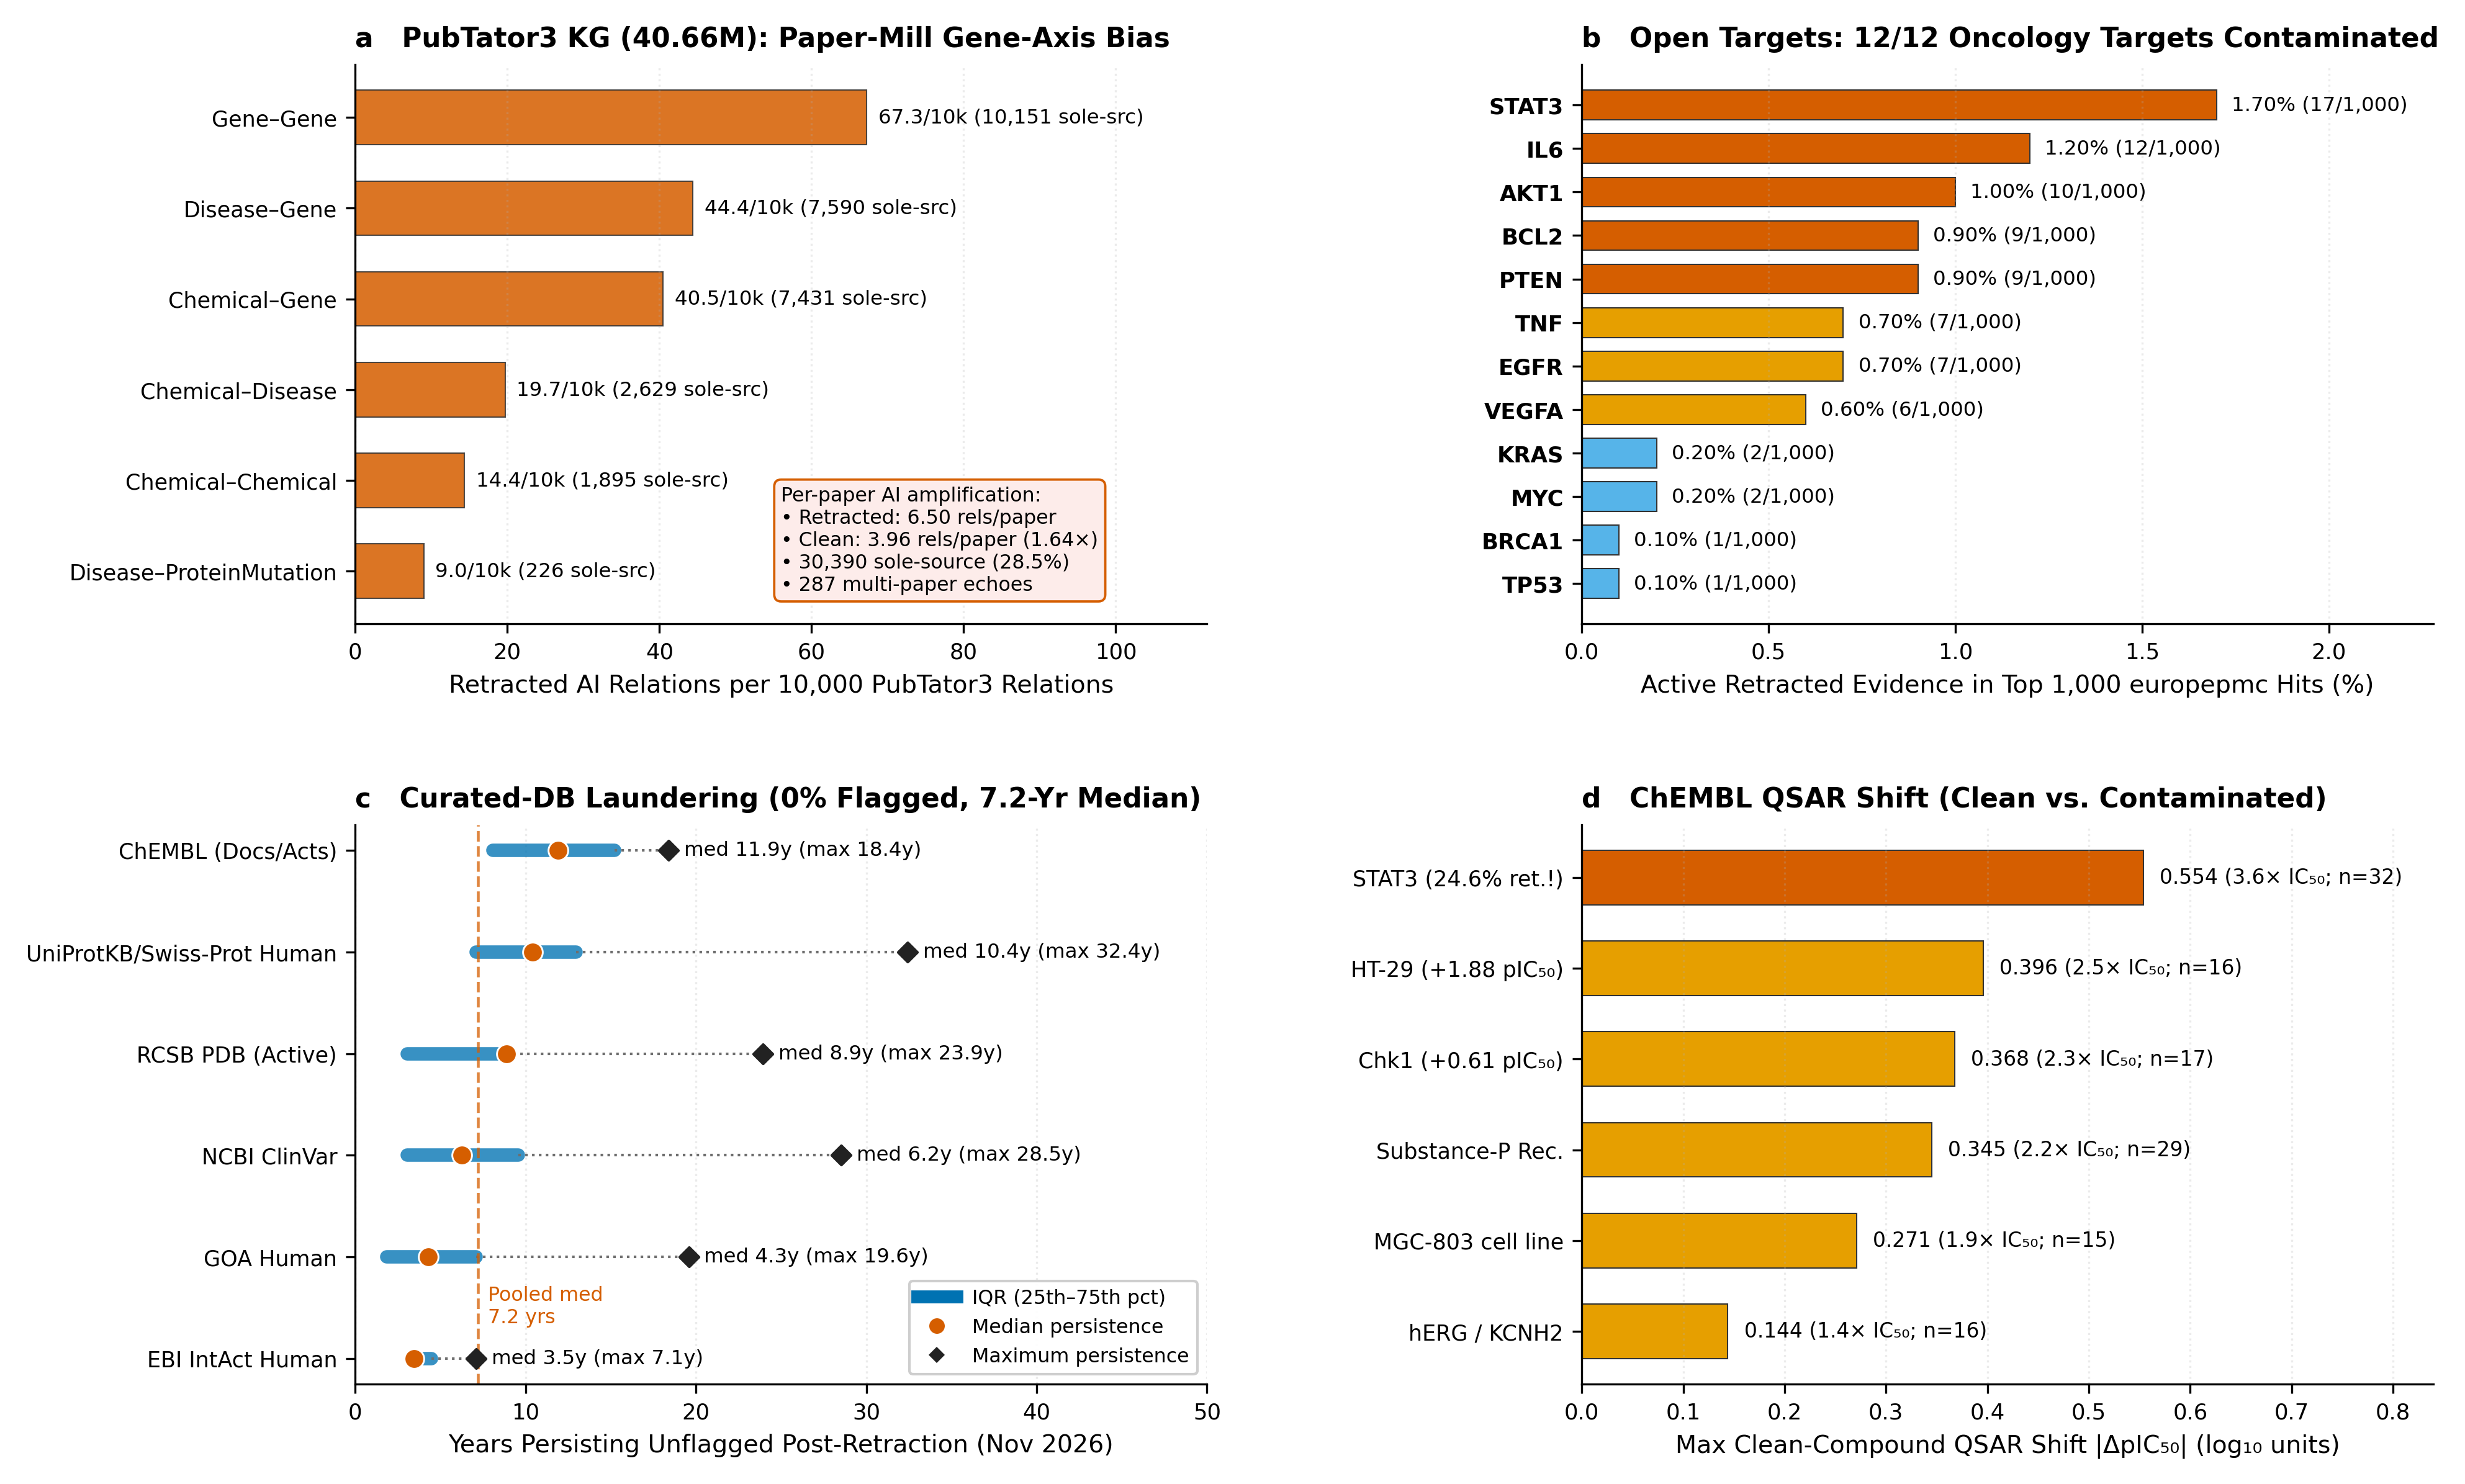
\includegraphics[width=\textwidth]{figures/fig3_pubtator3_kg_and_curated_persistence.png}
\caption{\textbf{Automated AI knowledge graph poisoning versus multi-decade curated-database laundering and ChEMBL QSAR distortion.} \textbf{a}, PubTator3 retracted relation rates per 10,000 by entity-type pair and counts of 100\% sole-source retracted triples ($N=30{,}390$). \textbf{b}, Active unflagged retracted \texttt{europepmc} evidence in Open Targets Platform across 12 canonical oncology targets (12/12 contaminated). \textbf{c}, Unflagged post-retraction persistence distributions (IQR bars, red median dots, black maximum diamonds; pooled median 7.20 years) across six human-curated databases. \textbf{d}, Maximum single-compound clean QSAR $|\Delta\mathrm{pIC}_{50}|$ prediction shift caused by retaining retracted ChEMBL bioactivities across the six highest-volume targets.}
\label{fig:kg_curated}
\end{figure}

\subsection{Clinical Trial Event-Study, ClinicalTrials.gov Silence, and \texttt{RetractionGuard}}
Finally, we audited the complete PubMed clinical evidence stack: \textbf{1,512 clean retracted clinical trials/RCTs}, \textbf{897 retracted meta-analyses/systematic reviews}, and \textbf{29 retracted clinical guidelines}. Matching 100.0\% (1,512/1,512) of retracted RCTs to NIH iCite yielded exact annual citation trajectories (\texttt{citedByPmidsByYear}) for 1,230 dated trials retracted $\le 2024$ (Fig.~\ref{fig:clinical}a). Overall, \textbf{968/1,230 (78.7\%)} accrued \textbf{9,802 strict post-retraction PubMed citations} ($\text{year} > \text{retraction year}$), including 1,265 NIH-classified clinical citing articles. In a paired event-study centered on retraction year $t=0$, mean annual citations fell by only \textbf{37.1\%} from pre-retraction years $t\in\{-2,-1\}$ to post-retraction years $t\in\{+1,+2\}$ (2.95 to 1.86 citations/yr; $N=1{,}136$, paired Wilcoxon $p=2.62\times 10^{-12}$); by years $t\in\{+3,+4,+5\}$, trials still averaged 1.25 citations/yr ($-64.8\%$), and \textbf{30.8\% remained actively cited at year $+8$}.

Auditing all 9,189 unique post-retraction citing PubMed articles identified \textbf{1,571 citation edges} from 563 retracted RCTs into \textbf{1,186 active non-retracted meta-analyses/systematic reviews} and \textbf{88 active non-retracted clinical practice guidelines}, cited a median of 3.0 years (max 33 years) after retraction (Fig.~\ref{fig:clinical}b). Title/abstract inspection confirmed that \textbf{100.0\% (88/88)} of these guidelines and \textbf{99.3\% (149/150 sampled)} of these meta-analyses contain no mention of ``retract'', ``fraud'', or ``misconduct'' in their title or abstract. Critically, this cascade is not driven solely by retracted-and-republished protocol-error trials such as PREDIMED (PMID 23432189): excluding PREDIMED leaves \textbf{8,887 post-retraction citations}, \textbf{1,120 active meta-analyses/SRs}, and \textbf{78 active guidelines}, while restricting strictly to permanent \textbf{fraud, data fabrication, image manipulation, and peer-review-ring RCTs} ($N=445$) still yields 73.26\% post-retraction citation prevalence (\textbf{1,929 post-retraction citations}, \textbf{246 active meta-analyses/SRs}, and \textbf{16 active guidelines}, including 15 meta-analyses and 3 guidelines citing the fabricated \emph{Lancet} Jikei Heart Study, PMID 17467513).

Extracting ClinicalTrials.gov NCT numbers from PubMed XML across all 1,512 retracted RCTs recovered 145 RCT--NCT links (144 live NCT records retrieved via ClinicalTrials.gov API v2). Of 134 NCT trials still listing the retracted PMID directly in \texttt{referencesModule}, \textbf{81/134 (60.4\%)}—and \textbf{91/144 (63.2\%)} of all linked NCTs—never mention ``retract'' anywhere in the entire \texttt{protocolSection} JSON (Fig.~\ref{fig:clinical}c); the remaining 39.6\% only display the word passively when an imported PubMed citation string happens to embed ``Retraction''.

To demonstrate that cross-layer retraction blocking is immediately feasible at negligible engineering cost, we built and benchmarked \textbf{\texttt{RetractionGuard}} (\texttt{scripts/retraction\_guard.py}), an open-source $O(1)$-memory streaming filter combining Crossref Retraction Watch and PubMed \texttt{Retracted Publication[pt]} (excluding reinstatements) with JATS XML metadata parsing (Fig.~\ref{fig:clinical}d). \texttt{RetractionGuard} loads all 37,692 PMIDs and 62,559 DOIs in \textbf{0.13 seconds}, stream-filters all \textbf{40,657,168 PubTator3 relations in 23.5 seconds} (1.73 million rows/s; blocking 130,302/130,302 retracted triples), filters \textbf{5,175,401 ClinVar citation rows in 2.1 seconds} (2.46 million rows/s; blocking 95/95), and achieves \textbf{100.0\% (30/30) recall} on a live AWS S3 JATS XML stress test deliberately enriched with all five untagged XML records (25 caught via \texttt{<related-article>}, 5/5 untagged caught via external registry fallback), compared with 12.1\% detection by naive JATS text extractors.

\begin{figure}[t]
\centering
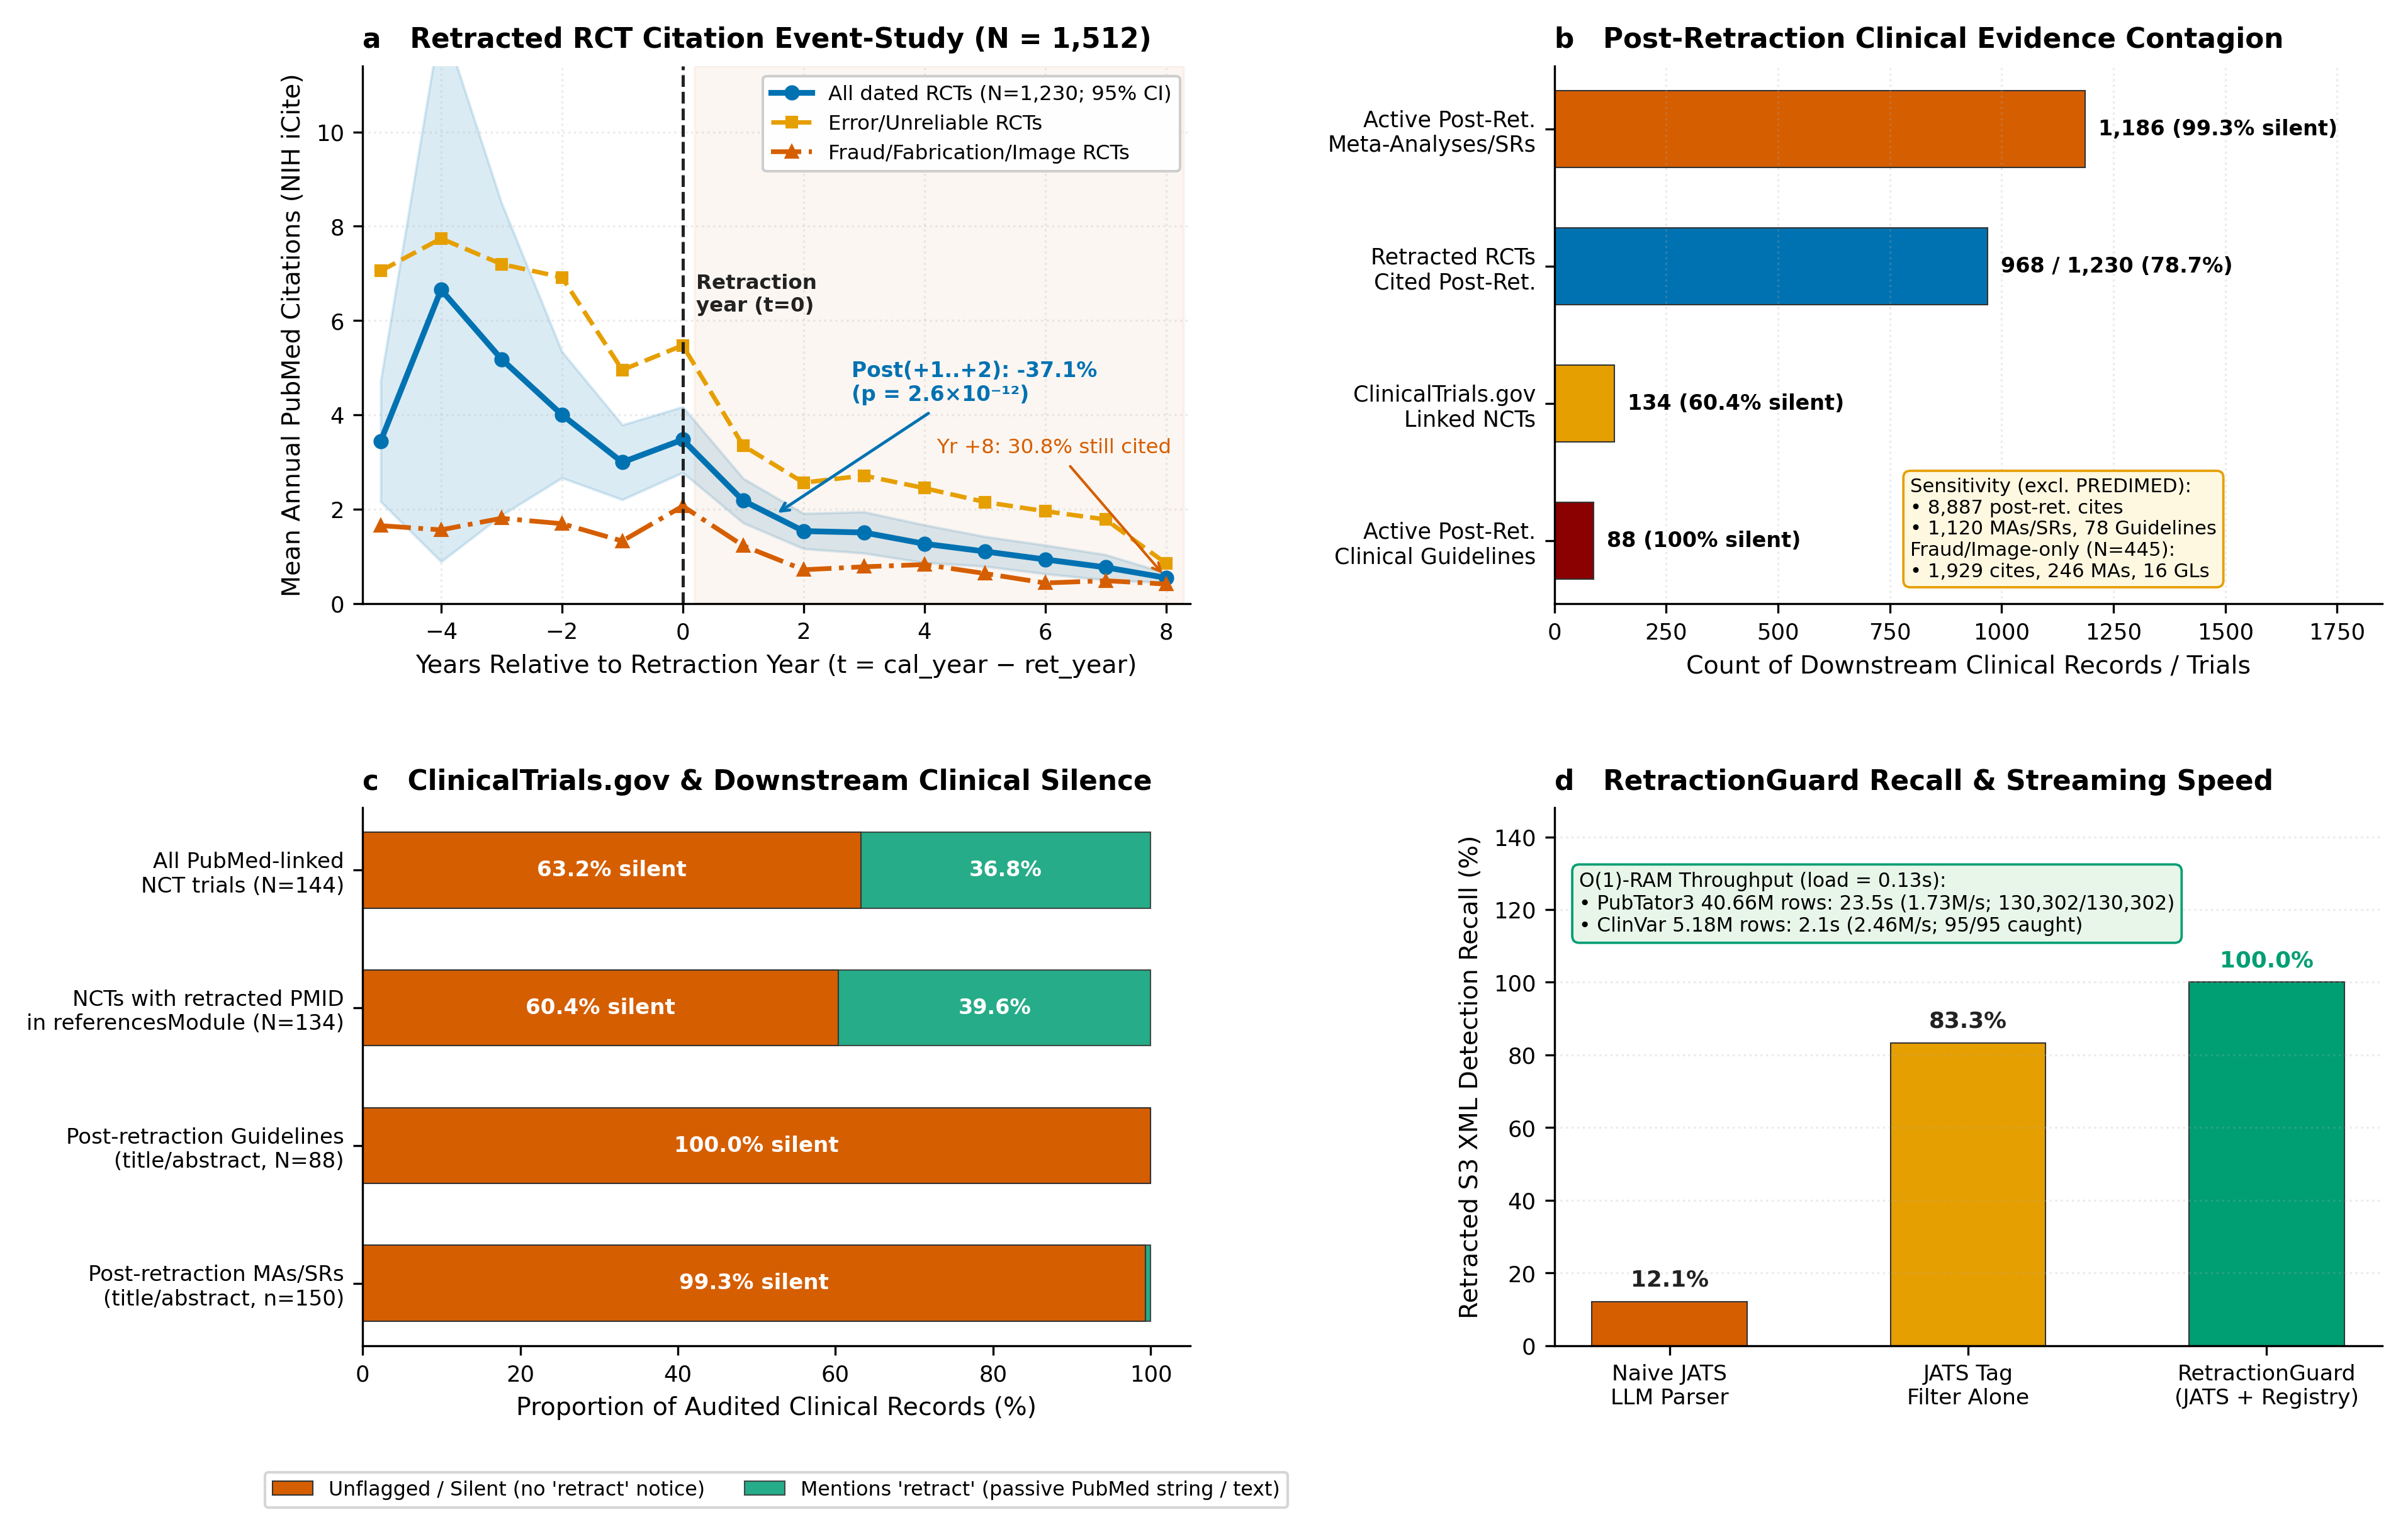
\includegraphics[width=\textwidth]{figures/fig4_clinical_cascade_and_retraction_guard.png}
\caption{\textbf{Clinical trial post-retraction citation event-study, ClinicalTrials.gov unflagged silence, and \texttt{RetractionGuard} defense.} \textbf{a}, NIH iCite event-study of mean annual citations ($\pm 95\%$ CI band) around retraction year $t=0$ across 1,230 dated retracted clinical trials, stratified by error/unreliable versus fraud/fabrication/image manipulation. \textbf{b}, Downstream post-retraction clinical contagion with PREDIMED-excluded and fraud-only sensitivity benchmarks. \textbf{c}, Unflagged silence rates across live ClinicalTrials.gov NCT records ($N=144$) and post-retraction clinical guidelines/meta-analyses. \textbf{d}, \texttt{RetractionGuard} JATS XML recall (30/30 = 100.0\%, including 5/5 untagged files) and $O(1)$-memory streaming throughput on PubTator3 and ClinVar.}
\label{fig:clinical}
\end{figure}

\section{Discussion}
Our cross-stack audit exposes a structural blind spot at the heart of modern biomedical AI. Because human-curated databases such as ClinVar, RCSB PDB, and ChEMBL show low overall retracted fractions (0.002\%--0.023\%), it is tempting to assume retracted literature poses a negligible risk to computational biomedicine. That conclusion fails for two opposing reasons. First, inside human-curated databases, low entry prevalence coexists with near-total post-retraction neglect (0\% active flagging; 7.2-year median persistence), enabling decades-old retracted crystal structures to persist inside protein foundation-model training sets and allowing a single retracted paper to constitute one-quarter of all ChEMBL bioactivity data for an oncology target like STAT3. Second, and far more consequentially, as biomedicine shifts from manual curation to automated text-mining knowledge graphs and open-access LLM training, it discards human entry screening while introducing \emph{positive legal selection for paper mills}: filtering to PMC Open Access to avoid publisher copyright selects the exact stratum where retracted literature is $1.83\times$--$7.78\times$ enriched, while JATS XML parsing strips the metadata tags that distinguish retracted articles from valid research.

Several methodological boundaries warrant transparent emphasis. First, our prior-art novelty statement is bounded strictly to our documented November 25, 2026 searches across PubMed, Europe PMC, and OpenAlex. Second, in the clinical cascade analysis, automated PubMed citation-graph linkage and title/abstract screening cannot distinguish between a meta-analysis that uncritically pooled a retracted trial versus one that cited it solely in the Methods section to report its exclusion; full-text manual adjudication of all 1,186 meta-analyses and 88 guidelines remains important follow-up work. Third, 2025 PMC OA enrichment is right-censored by the 1.36-year median retraction lag, and protein-level prevalence in UniProtKB/Swiss-Prot (0.78\%) aggregates multiple references per protein and is therefore not directly comparable to single-row association rates in ClinVar or GWAS Catalog. Fourth, our ChEMBL QSAR benchmark demonstrates that global cross-validation RMSE metrics are insensitive to localized contamination; vulnerability concentrates in lower-data targets and structural analogs close to fabricated series.

The EBI GWAS Catalog's zero-retraction record (0/1,206,717) proves that active retraction governance is entirely achievable. We recommend four concrete infrastructure standards: (1) \textbf{Unified automated retraction synchronization} combining Crossref Retraction Watch (excluding reinstatements) with PubMed \texttt{Retracted Publication[pt]} on every monthly release of ClinVar, ChEMBL, UniProt, GOA, IntAct, RCSB PDB, PubTator3, and Open Targets—never relying solely on PubMed flags (which miss 1,865 Retraction Watch retractions); (2) \textbf{Explicit machine-readable retraction propagation} in JATS XML (\texttt{article-type="retracted-article"}) and ClinicalTrials.gov \texttt{referencesModule}; (3) \textbf{Mandatory pre-ingestion \texttt{RetractionGuard} filtering} before tokenizing PMC Open Access dumps for biomedical LLMs or constructing GraphRAG indexes; and (4) \textbf{Flagged archival retention rather than silent deletion} for clinical audit trails (such as ClinVar SCVs and PDB coordinates), ensuring historical transparency while excluding retracted assertions from active clinical decision support and AI training by default.

\section{Methods}
\subsection{Master Retraction Registry Construction}
We downloaded the official Crossref Retraction Watch CSV (\texttt{retraction\_watch.csv}, SHA-256 \texttt{6db839a1b0a8...}, 74,070 rows; 68,607 rows with \texttt{RetractionNature == "Retraction"}) and identified all rows containing ``Reinstate'' in \texttt{RetractionNature} (136 unique PMIDs; 160 unique DOIs), which were excluded from every downstream registry and database join. To avoid NCBI ESearch's 9,999-record \texttt{retstart} ceiling, we partitioned \texttt{Retracted Publication[pt]} and \texttt{Retracted Publication[pt] AND "pubmed pmc open access"[filter]} across 14 date windows (\texttt{1800--2004} through \texttt{2024--2026}, with 2022 split quarterly), recovering 35,847/35,847 (100.00\%) and 19,010/19,010 (100.00\%) reported PMIDs respectively. After removing reinstatements, the union of PubMed (35,827) and Retraction Watch (30,769) yielded 37,692 unique retracted PMIDs. Retraction Watch reasons were mapped hierarchically to six mutually exclusive mechanism classes: data fabrication or paper mill, image manipulation or duplication, peer-review manipulation, plagiarism or text duplication, error or unreliable results, and other misconduct or administrative causes.

\subsection{PMC Open Access Enrichment and Live AWS S3 JATS XML Audit}
Year-by-year counts (2010--2025) of total PubMed articles, PMC OA articles (\texttt{"pubmed pmc open access"[filter]}), retracted PubMed articles, and retracted PMC OA articles were queried via NCBI ESearch on November 25, 2026. Exact $2\times 2$ odds ratios with Woolf 95\% confidence intervals, two-sided $\chi^2$ $p$-values, Wilson 95\% binomial intervals, and year-stratified Cochran--Mantel--Haenszel (CMH) odds ratios across 2010--2024 were computed before and after subtracting all Hindawi-published retractions by original publication year. For the live corpus audit, 240 retracted PMC OA PMIDs stratified across 2012--2024 were mapped to PMCIDs and fetched directly from \texttt{https://pmc-oa-opendata.s3.amazonaws.com/}. Each \texttt{.txt} and \texttt{.xml} object was parsed to check \texttt{article-type}, \texttt{<related-article>}, and case-insensitive occurrence of ``retract'' inside standard LLM text-extraction nodes (\texttt{<article-title>}, \texttt{<abstract>}, and \texttt{<body>}).

\subsection{AI Knowledge Graph, Curated Database, QSAR, and Clinical Cascade Audits}
We downloaded NCBI PubTator3 \texttt{relation2pubtator3.gz} (301.8 MB, November 17, 2026) and \texttt{mutation2pubtator3.gz} (111 MB) and ran a two-pass streaming scan to count exact retracted relations, per-paper extraction density, and sole-source retracted triples (canonicalizing symmetric relation types). Open Targets Platform GraphQL v4 was queried for the top 1,000 \texttt{europepmc} evidence rows per gene across 12 canonical oncology targets (\texttt{MONDO\_0004992}; \emph{BRCA1} against \texttt{MONDO\_0007254}). Eight human-curated databases were audited via official bulk releases or REST APIs (NCBI ClinVar \texttt{var\_citations.txt}, RCSB PDB Search/Core REST + wwPDB \texttt{obsolete.dat}, UniProtKB/Swiss-Prot Human, ChEMBL REST API, GOA Human \texttt{goa\_human.gaf.gz}, EBI GWAS Catalog full associations zip, CIViC evidence TSV, and EBI IntAct \texttt{human.zip}). Persistence was computed as $(\text{2026-11-25} - \text{RetractionDate})/365.25$. For ChEMBL QSAR perturbation, all clean and retracted pChEMBL records for the top six contaminated targets were featurized with 2,048-bit RDKit Morgan fingerprints ($r=2$) and evaluated under 5-fold cross-validated Ridge regression ($\alpha=10.0$) comparing clean-only versus contaminated training folds. Clinical trial event-studies used NIH iCite (\texttt{https://icite.od.nih.gov/api/pubs}) across all 1,512 clean retracted RCTs, paired Wilcoxon signed-rank tests, PubMed \texttt{esummary}/\texttt{efetch} publication-type and title/abstract screening across all 9,189 post-retraction citing articles, and live ClinicalTrials.gov API v2 queries across all 144 XML-linked NCT trials. All scripts, verified summary tables, and \texttt{RetractionGuard} are archived in the project repository.

\bibliographystyle{unsrtnat}
\bibliography{references_c2_zombie}
\end{document}
